\documentclass[conference]{IEEEtran}
\ifCLASSINFOpdf
  % \usepackage[pdftex]{graphicx}
  % declare the path(s) where your graphic files are
  % \graphicspath{{../pdf/}{../jpeg/}}
  % and their extensions so you won't have to specify these with
  % every instance of \includegraphics
  % \DeclareGraphicsExtensions{.pdf,.jpeg,.png}
\else
  % or other class option (dvipsone, dvipdf, if not using dvips). graphicx
  % will default to the driver specified in the system graphics.cfg if no
  % driver is specified.
  % \usepackage[dvips]{graphicx}
  % declare the path(s) where your graphic files are
  % \graphicspath{{../eps/}}
  % and their extensions so you won't have to specify these with
  % every instance of \includegraphics
  % \DeclareGraphicsExtensions{.eps}
\fi

\usepackage{booktabs} % For formal tables
\usepackage{multirow}
\usepackage{algorithm}
\usepackage[noend]{algpseudocode}
\usepackage[pdftex]{graphicx}
\usepackage[T1,hyphens]{url}
%\usepackage[colorlinks,urlcolor=blue]{hyperref}
\usepackage[]{hyperref}

\graphicspath{{./figures/}}
\algrenewcommand\textproc{}

%\algsetup{linenosize=\small}

% correct bad hyphenation here
\hyphenation{op-tical net-works semi-conduc-tor}

\begin{document}
%
% paper title
% Titles are generally capitalized except for words such as a, an, and, as,
% at, but, by, for, in, nor, of, on, or, the, to and up, which are usually
% not capitalized unless they are the first or last word of the title.
% Linebreaks \\ can be used within to get better formatting as desired.
% Do not put math or special symbols in the title.
\title{OBFS: OpenCL Based BFS Optimization on Software Programmable FPGAs}
% Ironing out the irregularity in BFS for efficient OpenCL implementation on Xeon-FPGA

% make the title area
\maketitle

% As a general rule, do not put math, special symbols or citations
% in the abstract
\begin{abstract}
    Breadth First Search (BFS) is a key building block of graph processing 
	and there have been considerable efforts devoted to accelerating BFS on FPGAs
	for the sake of both performance and energy efficiency. While prior work 
	typically built the BFS accelerator through handcrafted circuit design using 
	hardware description language (HDL). Despite the relatively good performance, 
	the HDL based design leads to extremely low design productivity, and incurs 
	high portability and maintenance cost. While the evolving high level synthesis (HLS) 
	tools make it convenient to create a functional correct BFS accelerator, 
	the performance of the baseline design remains much lower. 

	To obtain both the near hand-crafted design performance and the software-like features, 
	we propose OBFS, an OpenCL based BFS accelerator on software programmable FPGAs, 
	and explore a series of high-level optimizations to the OpenCL design. 
	With the observation that OpenCL based FPGA design is rather inefficient on 
	irregular memory access (random and short burst), we focus on the optimization 
	of irregular memory access in BFS. 
	First of all, we convert the low-efficient irregular edge reading into batched 
	memory access with graph reordering. Then we use an on-chip bitmap to avoid random 
	visiting status access over DDR. On top of the graph reordering and 
	on-chip bitmap, we further build conflict-free parallel data paths 
	to make best use of the on-chip memory bandwidth. In addition, we 
	shift the random BFS level update from the main BFS processing and 
	hide it with overlapped execution of different BFS processing. 
	According to the experiments on a set of representative graphs, 
	OBFS achieves up to 12X performance speedup compared to the reference design 
	in Spector benchmark on Intel Harp-v2. When compared to prior handcrafted design on 
	similar FPGA cards, it achieves comparable performance or even better on some R-MAT graphs. 
\end{abstract}

% For peer review papers, you can put extra information on the cover
% page as needed:
% \ifCLASSOPTIONpeerreview
% \begin{center} \bfseries EDICS Category: 3-BBND \end{center}
% \fi
%
% For peerreview papers, this IEEEtran command inserts a page break and
% creates the second title. It will be ignored for other modes.
\IEEEpeerreviewmaketitle

\section{Introduction} \label{sec:intro}
Inspired by the widespread adoption of neural networks in massive fields such as image classification, 
video surveillance, speech recognition, and robot vision, neural network accelerators 
\cite{Zhang2015_9,Qiu2016_10,deepburing_12,DiCecco_4,Zeng2018_18} 
are increasingly explored and deployed to improve the computing performance and energy efficiency.
Unlike generic applications, neural networks usually involve redundancy and are known to be 
fault tolerant\cite{Reagen2016}. By taking advantage of this feature, many neural network accelerator optimizations 
such as neural network pruning and low-precision quantization can be utilized to improve 
performance and energy efficiency notably with minor inference accuracy penalty\cite{Han2016DeepCC}. 

In line with these optimizations, we opt to relax the design constraints of 
the neural network accelerators, which provides a unique way to achieve notable 
improvements on performance or energy efficiency with small inference accuracy loss. 
For generic hardware design, strict design constraint is typically required to 
guarantee correct computing under even the most severe environments. On the contrast, 
neural network accelerators are more resilient and less sensitive to computing 
errors incurred by timing violations. Given relaxed design constraints, many 
aggressive hardware optimization techniques can be applied with computing errors. 
For instance, emerging techniques such as  near-threshold voltage regime\cite{RG2010NT} 
and subthreshold digital logic design\cite{BH2005,B2006} promise high energy efficiency 
but suffer instability\cite{Pu2010NT}. Conventional neural network accelerator 
can be pushed to operate at higher clock frequency with timing violations
\cite{overclock_3,Paceline_15}. At the fab level, design rules may also 
be aggressively pushed to reduce the expense. 

Motivated by the great advantages of relaxed design constraints,
we further explore the use of neural network resilience for more 
effective design trade-offs. When there are timing violations
and computing errors in the accelerator, the unmodified neural networks 
executed on the accelerators during inference is different 
from that computed on GPPs during the training, which may cause clear 
prediction accuracy loss. Instead of deploying the unmodified neural 
network models on the accelerators directly, we borrow the retraining 
idea from prior neural network quantization work \cite{Hwang2014_17,Matthieu2014_8} 
and have the deep neural network models to learn and tolerate the computing errors.  
Basically, we have the forward computing performed on the accelerator and 
then transfer the computing results to the host processor for 
backward propagation. With this approach, both application data and computing 
errors are learned and incorporated in the neural network models.  
Meanwhile, we define a set of standard interfaces to make it convenient 
to integrate general CNN accelerators into the retraining framework. 

In addition, we notice that some of the neural network layers are more sensitive to the 
computing errors and the sensitive layers dramatically limit the usefulness of the retraining. 
Thus, we schedule the most sensitive layer which is usually the last 
layer of the neural networks to host processors to reduce the negative influence 
of the computing errors. With both the retraining and sensitive layer protection, 
the neural networks become more resilient to the computing errors caused by 
the aggressive design options such as near-threshold logic or overclocking.
Compared to the original neural networks, the prediction accuracy of top-1 and top-5 
improves by 22.8\% and 9.89\% on average. The contributions of this work are 
summarized as follows.

\begin{itemize}
	\item We propose to improve the fault-tolerance of neural networks and make use of it to relax 
		the accelerator design constraints for higher performance or energy efficiency.

	\item We propose a neural network training framework to obtain resilient neural network models. 
		By integrating accelerator into conventional training, we have the computing errors 
		learned with the application data. By protecting the layer with most large errors, 
		we can further improve the resilience of the neural networks and pose more 
		opportunities to hardware optimizations.

	\item With comprehensive experiments, we show that the proposed training framework 
		could enhance the prediction accuracy of neural networks significantly 
		when the accelerators run with computing errors incurred by either 
		overclocking or lower voltage.
\end{itemize}
The paper is organized as follows. Section II analyzes the influence of 
the CNN accelerator computing errors on the neural network prediction accuracy. 
Section III presents the proposed training for neural networks executed on accelerators with computing errors.
Section IV demonstrate the use of the training on accelerators with overclocking and generic computing errors. 
Section V briefs the related work and Section VI draws the conclusion. 



\section{Background} \label{sec:background}
In this section, we will briefly introduce the high level FPGA design tools,
the widely used BFS algorithm and the baseline pipelined BFS structure 
as the background.

\subsection{High level FPGA design tools}
Despite the relatively good performance, 
the HDL based design typically results in low design productivity, large reuse, 
portability and maintenance cost as well as ease of use challenge. 
To address this problem, the FPGA vendors have started 
to offer high level programming options such as C/C++ and OpenCL, which makes 
it possible for the designers without much low-level circuit design 
experiences \cite{nimbix, xilinx-sdaccel, intel-opencl} 
to program the FPGAs efficiently. In addition, the accelerator 
described with high level languages preserves many software-like features 
such as portability, ease of maintenance and use. Considering the  
continuously growing FPGA resources and stringent time-to-market requirements, 
the high level FPGA design tools \cite{Nane2016hls-survey} get increasing popularity.

\subsection{BFS Algorithm}
BFS is a widely used graph traversal algorithm and it is the basic 
building component of many other graph processing algorithms. 
It traverses the graph by processing all vertices with the same distance from the 
source vertex iteratively. The set of vertices which have the same distance from the 
source is defined as frontier. The frontier that is under analysis in the BFS iteration 
is named as current frontier while the frontier that is inspected from current frontier 
is called next frontier. By inspecting only the frontier, BFS can be implemented efficiently 
and thus the frontier concept is utilized in many BFS implementations.

A widely used frontier based BFS algorithm implementation is named as 
level synchronous BFS \cite{attia2014cygraph, betkaoui2012reconfigurable, 
zhang2017boosting}. The basic idea is to traverse the frontier vertices 
and inspect the neighbors of the current frontier vertices to obtain the 
frontiers in next BFS iteration. Then the algorithm can start a new 
iteration with a simple switch of current frontier queue and next frontier queue. 
The algorithm ends when the frontier queue is empty.

\subsection{Baseline pipelined BFS}
The basic pipelined BFS structure with classical top-down traverse 
is presented in Figure \ref{fig:base-bfs}. It can be roughly 
divided into four pipeline stages. In the first stage, it reads 
frontier from memory. Then it passes the frontier to the second stage
via the OpenCL channel for further inspection. In the second stage, 
frontier neighbors will be inspected from the graph data. While the 
graph is stored as compressed sparse row (CSR) format which has a row 
pointer array (RPA) containing the edge index starting position of each 
vertex and a column index array (CIA) which is essentially the incoming/outgoing 
neighboring vertex indices, the second stage must go through the RPA read and 
CIA read sequentially. When the frontier neighbors are 
drained from memory, the second stage then forwards them to the third stage.
In the third stage, each neighboring vertex will be checked if it is 
already visited in previous BFS iterations. If the vertex is not visited, 
it will be considered as frontier in next BFS iteration. The corresponding 
vertex status will be set and the vertex index will be sent to the last stage.
In the last stage, the vertex indices of the next BFS frontier will be 
written to main memory and level of the frontier vertices will be updated.

\begin{figure}
\center{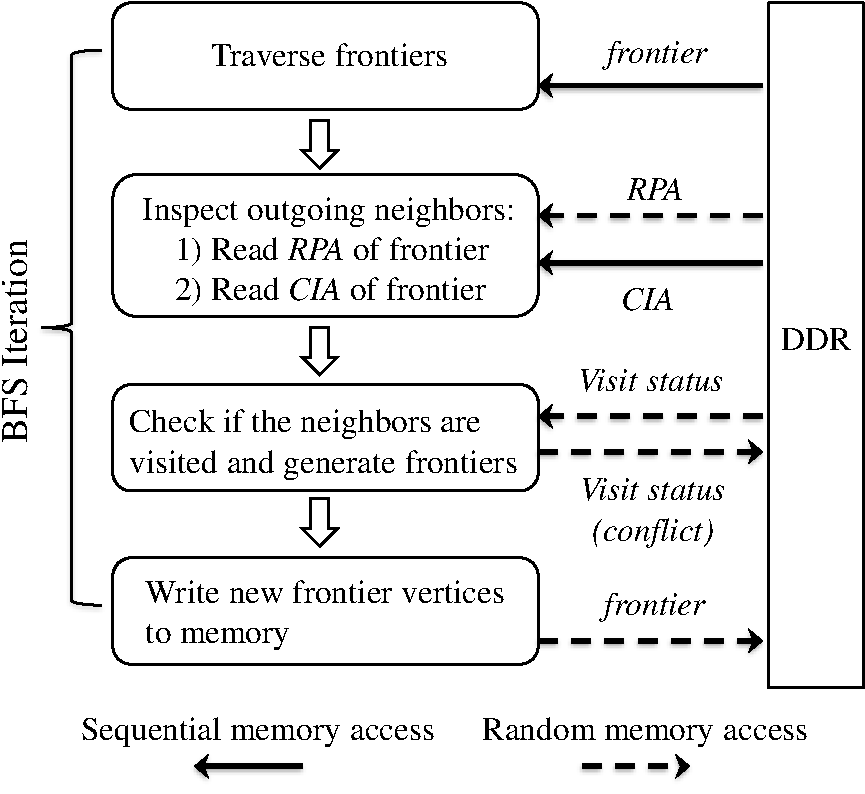
\includegraphics[width=0.7\linewidth]{base-bfs}}
    \caption{Baseline pipelined BFS}
\label{fig:base-bfs}
\vspace{-1em}
\end{figure}


 
\section{Motivation} \label{sec:motivation}
Clock frequency determines the accelerator operation speed 
and directly affects the performance. Accordingly, it also has influence on the 
neural network runtime and energy efficiency. In this section, we take 
an open-sourced CNN accelerator named PipeCNN \cite{pipecnn_2} as an example and analyze its 
influence on the neural network performance and energy efficiency.

The accelerator is implemented on KCU1500 and attached to a desktop computer with 
Intel i7-6700@3.40GHz. The basic convolution structure is shown in Fig \ref{fig:cnn-arch}. The largest computing 
array that can be accommodated by the FPGA device consists of 16 dot production units. 
Each dot production unit allows parallel processing of two 8-data vectors.
The accelerator consumes over 11\% LUT of the FPGA device. The optimized clock frequency 
according to the SDAccel compilation is 200 MHz. 

\begin{figure}
	\center{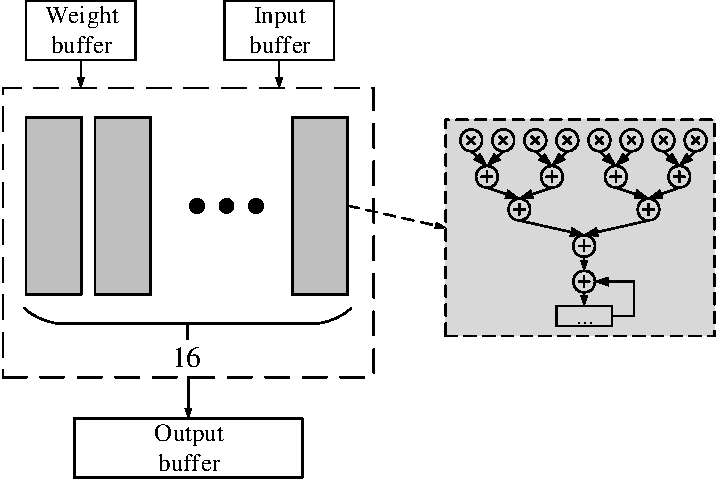
\includegraphics[width=0.75\linewidth]{accelerator}}
    \caption{Baseline CNN accelerator architecture.}
\label{fig:cnn-arch}
\vspace{-1em}
\end{figure}


In order to evaluate the influence of clock 
frequency, we further set the clock to 50 MHz, 100 MHz, and 150 MHz respectively.
A set of neural networks including LeNet, AlexNet, VGG-16 and VGG-19 are used as the benchmark.
Normalized performance the neural network benchmark executed on the accelerators are 
shown in Fig \ref{fig:computing-bound}. It can be found that the 
overall performance of the neural network benchmark
almost increases proportional to the clock frequency. For the larger neural networks, 
the processing remains the computing bound and high frequency design is highly demanded.

\begin{figure}
	\center{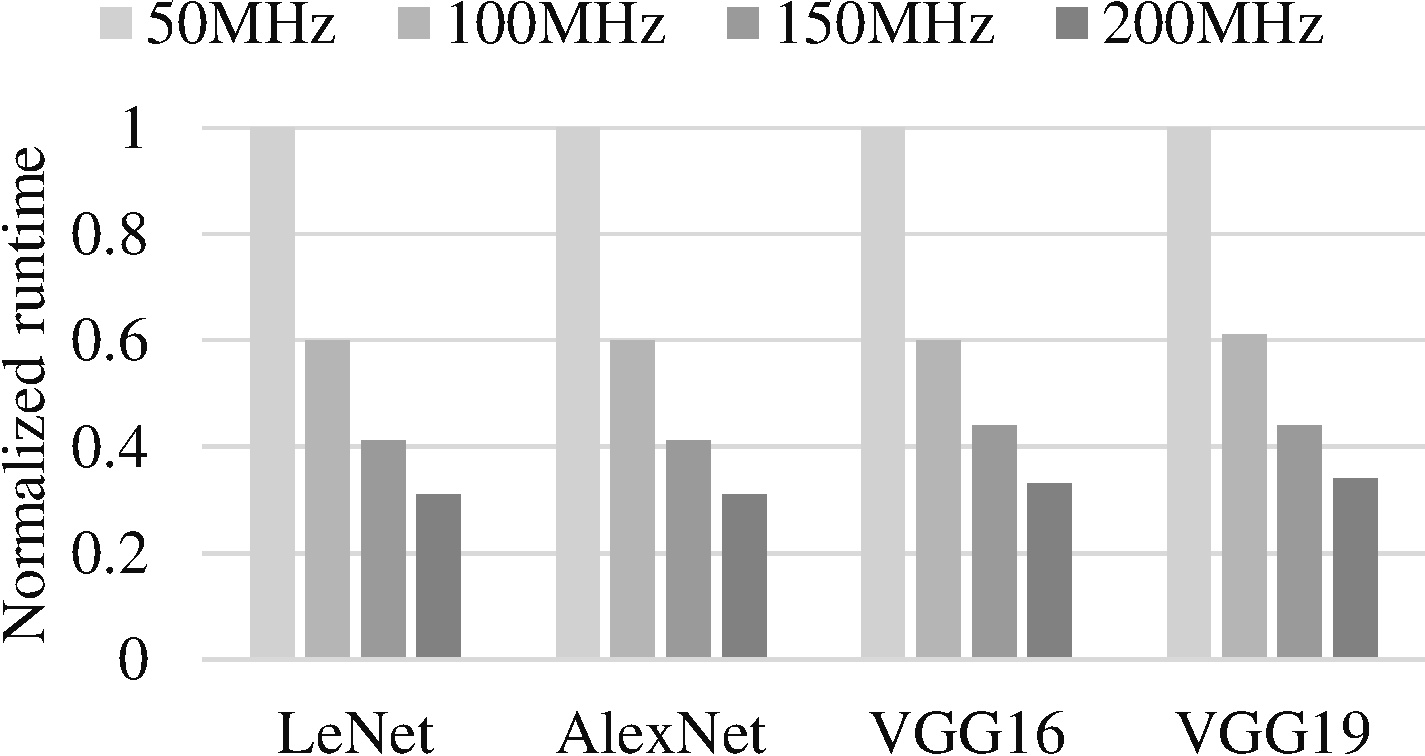
\includegraphics[width=0.75\linewidth]{relative_time}}
    \caption{Normalized performance of neural networks executed on CNN accelerators with different clock frequency.}
\label{fig:computing-bound}
\vspace{-1em}
\end{figure}

In addition, we also obtain the power consumption from SDAccel report. 
The power estimation setup assumes xxxx. Given the power consumption and the performance, 
we calcualted the energy delay product which can be used as an energy efficiency metric.
The energy efficiency is presented in Fig \ref{fig:edp}.
\begin{figure}
	\center{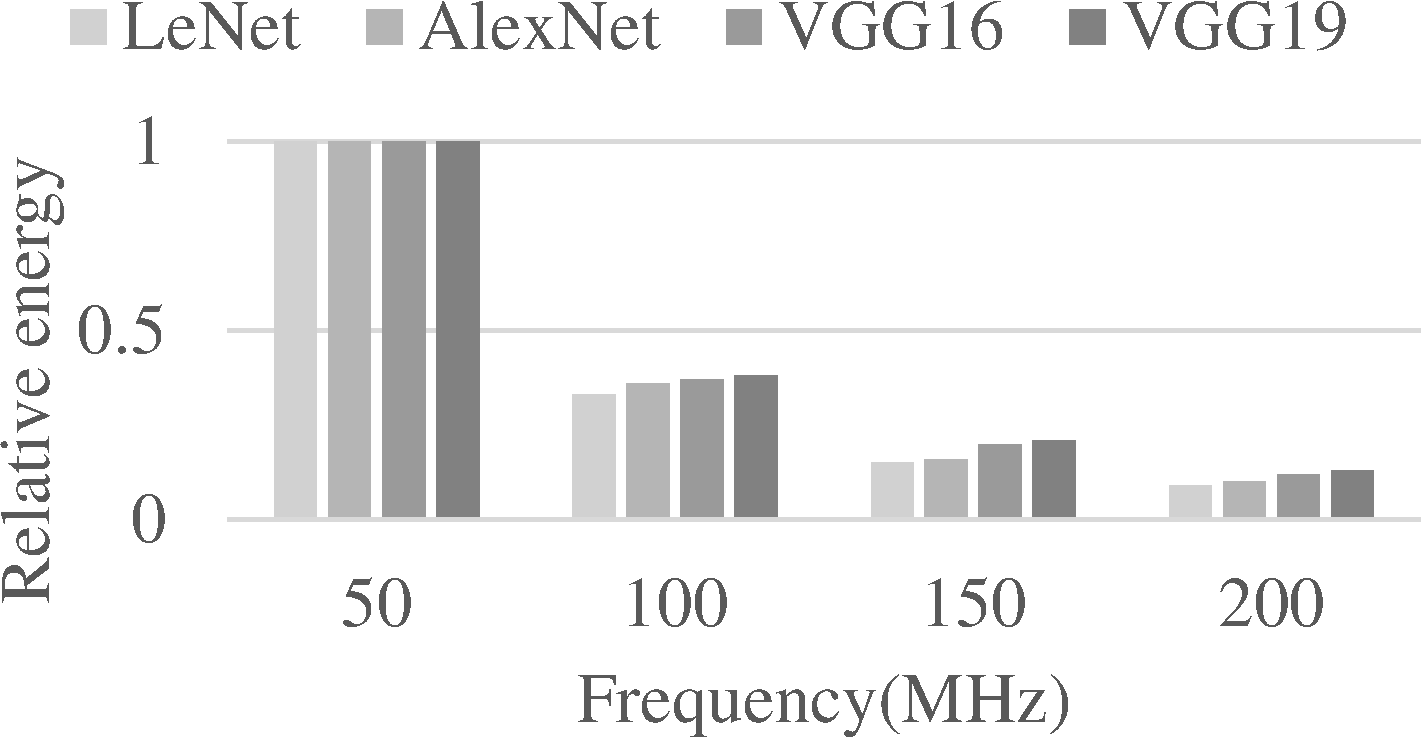
\includegraphics[width=0.75\linewidth]{relative_energy}}
    \caption{Normalized energy-delay product of neural networks executed on CNN accelerators with different clock frequency.}
\label{fig:edp}
\vspace{-1em}
\end{figure}

According to the above experiments, it can be conclcuded that higher clock frequency 
can be beneficial to both the neural network performance and energy efficiency. The 
potential performance and energy efficiency improvement indicates that it is 
worthwhile to boosting the clock of FPGA based CNN accelerators with some minor 
overhead. Detailed overclocking on CNN accelerators will be investigated in 
detail in the rest part of this paper. 

\section{HLS based BFS optimization} \label{sec:bfs-opt}
BFS is a system.
We need optimize the whole system from pre-processing to hardware pipelining.
This work centers the FPGA acceleration but it also needs assitance of a coupled CPU 
which can either be connected via PCIE or a shared memory structure.
We works on CSR data. irregular memory access? random memory accesses -->low bandwidth.
 memory access conflict, it is difficult to resolve the conflict using HLS. 
Try to explore on-chip memory bandwidth. We use bitmap to store the vivsiting status.
A single FPGA nowadays can already accommodate Graphs with millions of nodes.
pipelined BFS structure.

\begin{itemize}
\item pre-processing, graph reordering and padding
\item on-chip buffering and parallel data path II = 2
\item batch write
\item CPU assisted data reorganization
\end{itemize}

presents the overview of 
the BFS accelerator. It targets in-memory graphs on a PCIe based 
high performance FPGA card. The whole graph is stored in FPGA device 
memory with a standard CSR format. 
Ideally, the accelerator does the BFS on FPGA without 
any interference from the host CPU. However, we organize the accelerator 
following the data flow model of Xilinx HLS and the data flow model 
doesn't allow feedback from the downstream stages to previous stages.
(Detailed BFS data flow will be illustrated in the next section.)
As a result, we can only put one BFS iteration on FPGA while 
leaving the iterative execution control to the host CPU. In each BFS iteration, 
the BFS kernel on FPGA returns the BFS frontier size to host such that the host will 
decide if another BFS iteration should be invoked. Although short communication 
between the host and FPGA in each BFS iteration is needed, the communication cost 
is negligible compared to the execution time. Hereby, 
the overall BFS runtime is barely affected.

The BFS algorithm is critical to the BFS accelerator and we explore the 
existing level synchronous BFS algorithm in detail. We notice that 
the level synchronous BFS algorithm may have redundant vertices pushed to the 
frontier queue in a parallel architecture especially when the frontier grows larger.
The main reason roots in the large amount of overlapped neighbor vertices among the 
frontier vertices as mentioned in previous section. When the frontier neighbors 
are inspected in parallel for faster BFS traverse, these overlapped vertices may be 
considered as frontiers independently and inserted into the next frontier queue. 
As a result, there may be redundant vertices put into the frontier queue and it is 
rather complex to get rid of the redundancy \textit{completely}. Although the redundant 
vertices in the frontier will not cause any BFS mistakes, they will soon lead to large 
amount of redundant traverses recursively and degrade the BFS performance.

To address this problem, we analyze the frontier from the 
vertex status in each BFS iteration to completely cut down the 
propagation of the redundant frontier vertices as proposed in prior 
GPU based BFS acceleration \cite{liu2015enterprise}. The modified algorithm is described 
in Algorithm \ref{alg:modified-bfs}. Instead of inspecting on the frontier vertices directly, 
it starts with vertex status analysis and inspects the frontier 
in each BFS iteration. Although it seems the additional frontier inspection stage 
brings more memory access, the inspection processing are complete sequential 
memory access and can be done efficiently. It is still worth for the overhead 
when compared to the cost caused by the redundant frontier vertices. 
The rest part of the algorithm from line 10 to 15 is 
quite similar to the level synchronous BFS except that the frontier queues 
are no longer needed.


With the observations in Section \ref{sec:observation} 
and the modified BFS algorithm in Section \ref{sec:overview}, 
we start to optimize the BFS accelerator using high level design tools 
from a series of different angles. First of all, we convert the nested loop structure 
of the BFS to be a stream manner such that it can be fit into the data flow model in
Xilinx HLS for efficient pipelined execution. Then we explore a series of memory optimization 
techniques based on the BFS memory access characteristics observed in \ref{sec:observation}. 
Afterwards, we further apply some general HLS optimizations to the resulting design. Finally, 
we manually tune the design parameters such as the prefetch buffer size and cache size through 
the fast software emulation and provide optimized configurations for each graph data set.

\subsection{BFS pipelining}
The baseline BFS algorithm is a multi-level nested loop with 
dynamic memory accesses. It is quite challenging for the HLS 
tools to produce optimized hardware by adding the HLS pragmas to 
the native high level code directly because of the following two 
reasons. First of all, inner most loop and outer loop body can't be pipelined 
automatically by the HLS tools unless the inner most loop is fully 
unrolled and pipelined. Nevertheless, the inner most loop in BFS 
can't be fully unrolled because of the dynamic loop structure.  
Secondly, the outer loop nests access memory randomly even though 
these accesses are actually sequential because they must wait 
for the execution of the inner loop nest which can't 
be fully pipelined. This will lead to low 
memory bandwidth utilization. Similar problem also happens when the 
loop body is complex and different parts of the loop body fail to be 
pipelined properly. In summary, applying HLS pragmas to the native high level BFS code 
will produce low efficient design and the performance of the resulting hardware 
can be far from satisfying.  

To address these problems, we divide the BFS algorithm into pipelined 
sub functions. Basically, there are generally two rules that 
we can create pipelined functions. 
First of all, each loop nest can be packaged into a sub function 
and the dependent sub functions can be pipelined. There are four loop 
nests in Algorithm \ref{alg:modified-bfs}, 
but the loop in line 12 actually include two loops as we need to go through 
both the CSR row and column to obtain a frontier neighbor's index. Thus we 
actually have five sub functions following this rule. Secondly, complex loop body 
can be split to more fine-grained sub functions such that the dependent parts can 
be executed in parallel with additional buffers between them. 
In BFS inner most loop, we can further divide the \textit{depth} read and write 
operations to two dependent sub functions. We can 
do more partitions and create even deeper pipelines, while there is no 
guarantee for always better performance and more hardware resources 
are usually required.

Following the two pipelining rules, we create a six-stage 
pipelined BFS algorithm as detailed in Algorithm \ref{alg:bfs-stream}. 
The six sub functions are labeled as f1 to f6 respectively. In f1, 
vertex status is read from FPGA DDR memory sequentially through a streaming port. 
When the vertex status is fetched, f2 inspects the status 
flowed from the stream buffer, decides the current frontier 
and dumps the frontier to the downstream pipeline. 
With the frontier stream, f3 can further fetch graph 
data stored as CSR. CSR includes a row pointer array (RPA) 
and a column index array (CIA), and they must be sequentially accessed. 
In f3, we combine each pair of RPA entry of the frontier as a construct 
and pass it to the next stream function f4. When f4 gets the RPA pair, 
it can read the CIA sequentially through a streaming port. 
When data in CIA stream which is essentially the potential 
next frontier vertices are received in f5, their vertex status 
will be checked by reading the vertex status array stored in DDR as well.
Only the vertices that are not visited yet will be further forwarded to the f6. 
In f6, the vertex status will be updated.

\begin{algorithm}
	\caption{Pipelined BFS Algorithm} \label{alg:bfs-stream}
    \small
	\begin{algorithmic}[1]
        \Procedure {BFS}{}
        \State $frontier\_size \gets 1$
        \State $level \gets 0$
        \While {$(frontier\_size > 0)$}
        \State $f1(depth, depth\_stream)$
        \State $f2(depth\_stream, frontier\_stream, level, frontier\_size)$ 
        \State $f3(frontier\_stream, CSR.RPA, RPA\_stream)$
        \State $f4(RPA\_stream, CSR.CIA, CIA\_stream)$ 
        \State $f5(CIA\_stream, depth, next\_frontier\_stream)$
        \State $f6(depth, next\_frontier\_stream, level)$
        \State $level \gets level + 1$
        \EndWhile
        \EndProcedure
        \State

        \Procedure{f1}{$depth$, $depth\_stream$}
        \For {$v \in V$}
        \State $depth\_stream << depth[v]$
        \EndFor
        \EndProcedure

        \Procedure{f2}{$depth\_stream, frontier\_stream, level, frontier\_size$}
        \State $frontier\_size = 0$
        \For {$v \in V$}
        \State $d[v] \gets depth\_stream.read()$
        \If {$(d[v] == level)$}
        \State $frontier\_stream << v$
        \State $frontier\_size++$
        \EndIf
        \EndFor
        \EndProcedure

        \Procedure{f3}{$frontier\_stream, CSR.RPA, RPA\_stream$}
        \While {$(!frontier\_stream.empty())$}
        \State $v \gets frontier\_stream.read()$
        \State $RPA\_stream << [CSR.RPA[v], CSR.RPA[v+1]]$
        \EndWhile
        \EndProcedure

        \Procedure{f4}{$RPA\_stream, CSR.CIA, CIA\_stream$}
        \While {$(!RPA\_stream.empty())$}
        \State $[begin, end] \gets RPA\_stream.read()$
        \For {${v \in CSR.CIA(begin, end)}$}
        \State $CIA\_stream << v$
        \EndFor
        \EndWhile
        \EndProcedure

        \Procedure{f5}{$CIA\_stream, depth, next\_frontier\_stream$}
        \While {$(!CIA\_stream.empty())$}
        \State $v \gets CIA\_stream.read()$
        \If {$(depth[v] == -1)$}
        \State $next\_frontier\_stream << v$
        \EndIf
        \EndWhile
        \EndProcedure

        \Procedure{f6}{$depth, next\_frontier\_stream, level$}
        \While {$(!next\_frontier\_stream.empty())$}
        \State $v \gets next\_frontier\_stream.read()$
        \State $depth[v] \gets level + 1$
        \EndWhile
        \EndProcedure

    \end{algorithmic}
\end{algorithm}

According to the description of the streamed BFS algorithm, we notice that 
five sub functions involve external memory access and they have quite different 
memory access patterns. The memory access patterns are summarized in 
Figure \ref{fig:bfs-stream}. f3 reads all the vertex status and 
it has a long sequential memory read. f2 reads the CSR row pointer of the frontier, 
and it reads two sequential words each time. f1 reads the CSR column index and the 
burst length depends on the vertex degree which varies in a large range. 
f4 and f5 involves vertex status reads and writes of the next frontier vertices.
As these vertices are not sequential, the HLS tools just take them as random access 
without any specific hints from the designers. 

\begin{figure}
\center{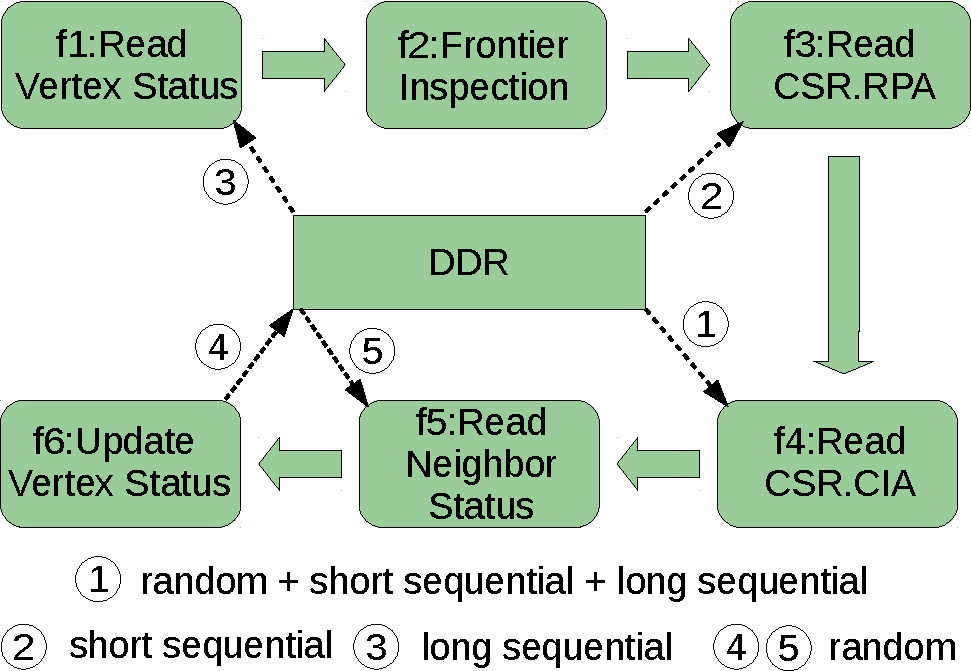
\includegraphics[width=0.65\linewidth]{bfs-stream}}
\caption{Streamed BFS Algorithm}
\label{fig:bfs-stream}
\end{figure}

\subsection{Memory Access Optimization}
As observed in Section \ref{sec:observation}, memory access especially the random and 
short sequential memory accesses are critical to the 
BFS performance. In this sub section, we will mainly explore the memory 
access optimization techniques based on the observations on top of 
the pipelined BFS design.

\subsubsection{Redundancy Removal}
There are many redundant vertices among the frontier neighbors in BFS. 
They may further cause unnecessary vertex status reads and writes in 
f5 and f6 respectively. In order to remove the redundant memory access 
and improve the memory bandwidth utilization, we create hash tables 
to perform the redundancy removal. As the redundant vertices are 
relatively random, a big hash table can be utilized to squeeze 
the redundancy. However, big hash table degrades the hardware implementation 
frequency and eventually lowers the overall performance. Hereby, we 
build a series of smaller hash tables and apply them in parallel. 
The hash table based redundancy removal structure is shown in Figure \ref{fig:hash-strategy}. 
We use the lower bits of the data address as the hash function 
for the sake of better timing. An input data that fails to find a 
record in any of the hash tables will be considered to be a unique 
data and put into one of the hash tables to avoid repeated data 
going through the filter. In order to ensure balanced hash 
table utilization, we implement a hardware-friendly round robin 
arbiter to decide the hash table updating order. 
  
\begin{figure}
\center{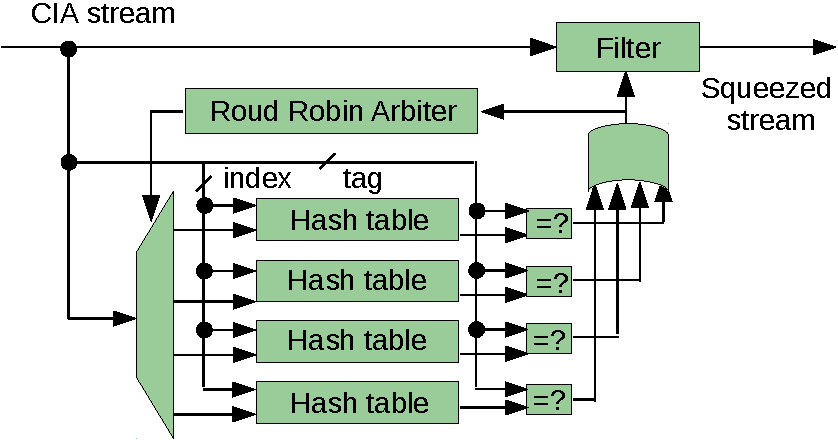
\includegraphics[width=0.75\linewidth]{hash-strategy}}
    \caption{Redundancy removal based on parallel hash tables.}
\label{fig:hash-strategy}
\end{figure}

\subsubsection{Caching}
According to the experiments in Section \ref{sec:observation}, 
there are many random memory accesses and short 
sequential memory accesses in f5 and f6. 
It is generally difficult to optimize these memory accesses. Fortunately, 
the spatial locality analysis shown in the observation experiments 
implies the great potential of cache based memory access optimization. 
Inspired by the observation, we developed an HLS based cache specifically 
for the vertex status \textit{depth} access. 

Since the cache is only used for \textit{depth} array read and write, we  
choose the \textit{depth} array index instead of its physical address for cache 
indexing. Each cache line is set to be 512-bit which is equal to the recommended 
memory access data width and a single memory read or write operation can 
fulfill the requirement of the cache operations including cache read miss, 
cache write miss and cache write back. Since the cache can't be shared 
between different SDAccel data flow functions, a natural cache design is 
to implement both cache in f5 and f6. Both cache can be relatively simple 
for supporting only read operations in f5 and write operations in f6.  

In this work, we choose the directly mapped cache for the BFS optimization. 
Cache line size is set to be 64B which fits well with the optimized global memory 
access port data width.
Although set associative cache architectures will achieve higher 
cache hit rate, the benefit is mostly compromised by the degraded 
implementation frequency on Alpha Data FPGA board. The trade-off 
may be different on a more advanced FPGA boards, but the optimization 
philosophy is pretty much similar. 
 
\subsubsection{Prefetching}
According to the BFS algorithm, the frontier is sequentially inspected. 
Therefore, the CSR information is also accessed in one direction 
in f3 and f4, though they are not necessarily sequential. Basically 
both the column array index and the row column index will increase 
monotonically in one BFS iteration. The CSR data will not be repeatedly 
referenced through the BFS. To optimize these memory 
accesses, a small prefetch buffer 
is build to improve the memory access efficiency. 

Prefetch buffer is also an important design parameter that needs to be tuned.
The general design trade-off is complex.
A larger prefetch buffer improves the hit rate, but it may incur more memory 
access cost and waste the memory bandwidth if the prefetched data are 
not fully used. Meanwhile, larger prefetch buffer adds prefetching cost 
when there is prefetch buffer miss, which may degrade the performance. 
A smaller prefetch buffer typically lead to lower hit rate though 
the prefetched data will be mostly used. Nevertheless, we notice that 
prefetching data that is smaller than 64B will not have clear advantages on timing 
nor memory bandwidth utilization compared to 64B prefetch buffer. 
On the other hand, prefetching more than 64B data doesn't have 
significant hit rate improvement and even results in 
performance drop mainly due to the increase of the prefetch cost when there 
is prefetch buffer miss. In this case, 64B is set to be the prefetch buffer size 
in the end.

\subsection{General HLS optimization}
On top of the pipelining, redundancy removal and caching, there are also 
many other relatively general design optimizations that can improve the 
resulting BFS accelerator performance. These optimizations will be briefly 
introduced in this sub section.

\subsubsection{Data path duplication}
When the DDR memory bandwidth is not saturated, a simple 
yet efficient optimization method is to duplicate the data paths. 
With multiple parallel BFS data paths, the accelerator can issue more parallel 
memory requests pushing higher memory bandwidth utilization. A straightforward 
way of data path duplication is to split the vertex status into different 
partitions and each partition is processed by an instance of the same BFS data path.

However, this method may not work as good as expected for three reasons. 
First of all, the vertices in the frontier may not distribute evenly across the graph. 
As a result, the different pipelines may have unbalanced workloads. Secondly, 
when the cache is applied to the pipelined data path, the same cache line may 
have multiple copies stored in f6 cache and this may cause 
cache coherence problem when they are modified differently 
and written back to memory independently. Finally, duplicating 
the non-bottleneck pipeline stages will not be beneficial to 
the final performance while it incurs more hardware resource consumption 
including not only the basic FPGA cells but also the global memory ports. 

To address the problems, we propose a delicate data path duplication strategy 
as shown in Figure \ref{fig:duplicate-pipeline}. According to the BFS algorithm, 
we know that each frontier vertex requires two CSR row pointer read and multiple 
CSR column index read. Thus the bottleneck pipeline stages may probably start 
from f3. In this case, we split the stream generated in f3 into 
multiple streams. Each sub stream will be handled independently by a 
duplicated data path. This also solves the data path load balancing problem 
naturally. Finally, to ensure a simple yet efficient cache coherence, we 
merge the output stream of f5 into a single stream before flowing into the 
last f6 stage with a write cache. 

\begin{figure}
\center{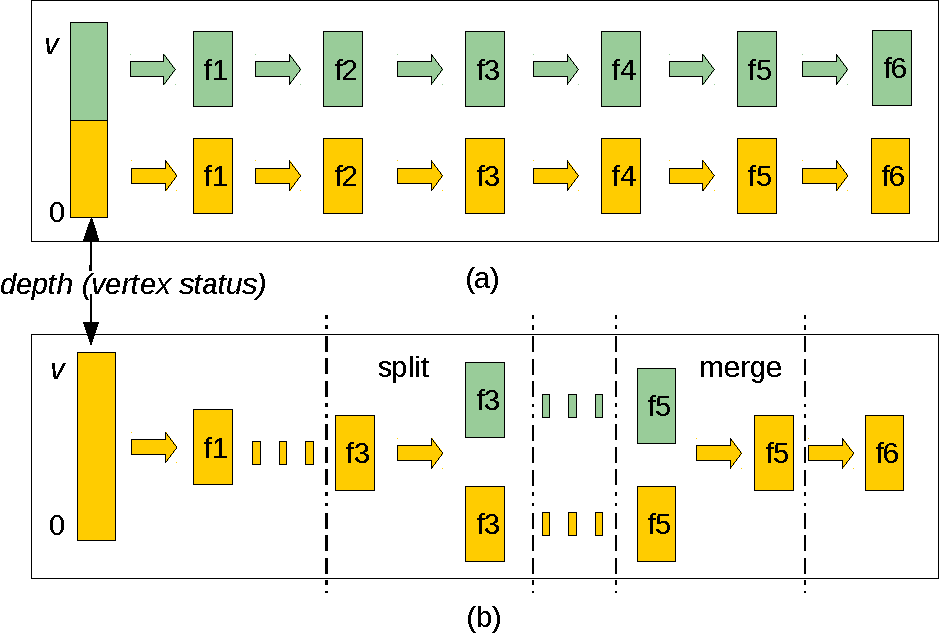
\includegraphics[width=0.85\linewidth]{pipeline-duplication}}
    \caption{pipeline duplication. (a) straightforward pipeline duplication 
    (b) optimized pipeline duplication.}
\label{fig:duplicate-pipeline}
\end{figure}


\subsubsection{Data width optimization}
The memory bandwidth utilization is sensitive to the data width setup. 
According to our experience, sequential memory access 
with 512-bit data width achieves the optimal memory bandwidth. With this guideline, 
a lot of design parameters such as the cache line size and prefetch length are 
set to be 512-bit for higher memory bandwidth utilization. For sequential 
memory access with smaller data width such as 32-bit, we must ensure that the 
data is aligned to 512-bit through padding the access. Otherwise, writing 
unaligned data may corrupt the data in memory.

%\subsubsection{II optimization}
%In the pipelined design, initialization interval (II) indicates the 
%processing throughput. Larger II in a single pipeline stage 
%may slow down the rest of the system. Thus we try to reduce II of all 
%the pipelined sub functions. In particular, hash table, cache and prefetch 
%buffer may affect the II. Inappropriate implementation may lead to 
%large II and even compensate the benefits brought by these optimizations. 

\subsubsection{Deadlock removal}
Another challenge of the pipelined BFS accelerator design is the 
unexpected deadlock problem. 
When a pipeline stage issues a long burst request to the memory 
but gets stalled due to the insufficient read buffer, it has to 
wait for the downstream pipeline stages to consume the data in the buffer. 
However, the downstream pipeline stages may also be stalled due to 
the failure of acquiring the bus that is taken by the upstream pipeline stage.
It is difficult to debug and resolve this deadlock. To address this problem, we
add additional user buffer in the pipeline stages with long sequential 
memory access and split the long sequential memory access into smaller 
segments such that each segment can be accommodated by the buffer. 
Although this may cause slightly lower bandwidth utilization, it breaks the deadlock and 
ensures the correctness of the pipelined design.

\subsection{Parameter Tuning}
As presented in previous sub sections, there are quite some design 
parameters such as hash table size and cache design, 
that need to be explored. However, exploring the design parameters 
based on the hardware implementation directly requires many lengthy 
hardware implementations (A typical BFS implementation may 
take 1 hour to 4 hours to complete.) which is extremely time-consuming.

In this work, we manually tune the design paramters. To obtain the optimized 
design parameters rapidly, we extract a series of hardware implementation independent 
metrics such as cache hit rate and hash table hit rate 
through faster software emulation mode in SDAccel which typically completes in a few minutes.
With these metrics, we can roughly decide the prefetch buffer size, 
cache size and hash table size etc. Afterwards, we go through the lengthy 
hardware implementation and choose the best parameters based on the final 
run time. A more systematic design parameter tuning will be helpful, but it 
is beyond the scope of this work and we will leave it for our future work.

%\subsection{Parameter tuning}
%In this work, we manually tune the design parameters. To obtain the 
%optimized design parameters rapidly, we proposed a general HLS design 
%parameter tuning flow for the HLS based design. The design flow is 
%presented in Figure \ref{fig:parameter-tuning}. It includes three 
%iterative loops tuning different types of the design parameters.
%
%The first loop replies on the fast software emulation which is 
%immediately available using HLS.
%With the software emulation, we can extract a set of statistical 
%metrics such as cache hit rate, prefetch hit rate that are 
%mostly independent with the hardware implementation. These metrics can be used to 
%guide the cache and prefetch buffer design. Although they 
%are not sufficient to decide the exact accelerator performance, they 
%can help prune the design options that are far from optimal and thus reduce 
%the design parameter tuning time. The second tuning loop is based on the hardware 
%pre-synthesis which is also fast and can be done in a few minutes. 
%With the pre-synthesis report, we can optimize the II by 
%improving the HLS design. When the potential design 
%configurations gets smaller, we can get into the last loop and start the time consuming 
%hardware implementation evaluating the configurations with the real 
%performance or resource metrics. Finally, we would like to emphasize the verification process, 
%it needs to be enabled all the time, as optimization may also cause mistakes of the resulting design.
%
%\begin{figure}
%\center{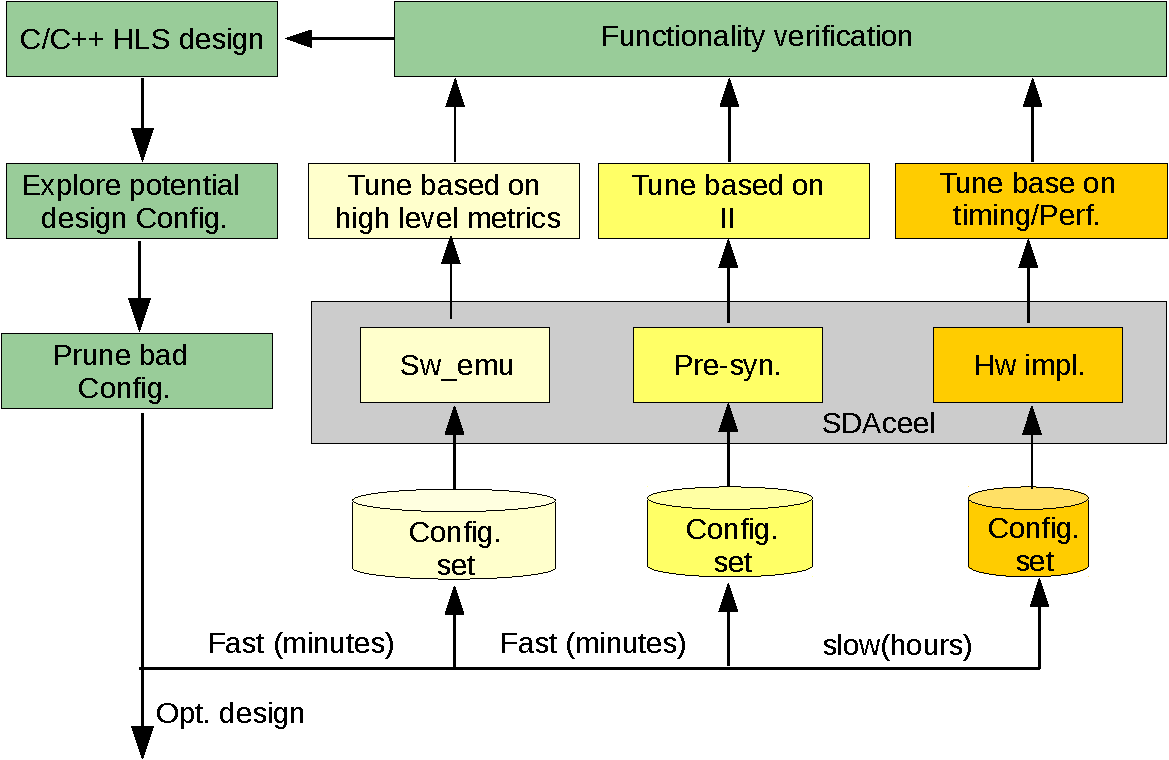
\includegraphics[width=0.95\linewidth]{parameter-tuning}}
%    \caption{Design parameter tuning flow based on SDAccel.}
%\label{fig:parameter-tuning}
%\end{figure}
%

%\appendix
%\section{Acknowledgement}

%\begin{acks}
%  The authors would like to thank Sam Ho for providing the suggestions on
%  HLS design debugging and optimization as well as the SDAccel usage. 

%\end{acks}

\section{Experiments}
In this section, we analyze the benefits of 
overclocking on a set of representative convolution neural networks.
and estimate the trade-offs of the strategies 
used to mitigate the overclocking incurred errors.

\subsection{Experiment setup}
We used PipeCNN as the baseline CNN accelerator and had it implemented on KCU1500 FPGA board.
Four representative neural networks including LeNet, AlexNet, VGG-16 and VGG-19 are used to 
benchmark the performance and energy efficiency of the CNN accelerator. The implementation clock
frequency of LeNet and AlexNet is 210 MHz while the clock frequency for VGG-16 and VGG-19 is 
190 MHz. Then we gradually overclock the implementation with 10 MHz step until the accelerator gets 
stuck or crashes frequently. For the 210 MHz implementation, the highest overclocking setup is 
260MHz. For the 190 MHz implementation, the highest overclocking setup is 240 MHz.
Finally, we evaluate the performance and energy efficiency of the accelerators using 
all the available overclocking configurations.

\subsection{Accuracy, performance and energy efficiency}
The prediction accuracy of the benchmark neural networks on the CNN accelerators with overclocking is 
presented in Fig \ref{fig:overclock-accuracy}. It can be found that the prediction accuracy 
regardless of top1 or top5 typically remains the same under moderate overclocking. However, when the clock 
continues to rise, it may reach to a tipping point where the prediction accuracy drops clearly. 
Fortunately, the prediction accuracy can be improved with just on-accelerator retraining.
When the clock further increases, the prediction accuracy drops dramatically. In spite of the retraining, 
the prediction accuracy is still not acceptable in practice. Part of the reasons can be that the 
number of timing violations increases rapidly with higher clock frequency. 
\begin{figure}
        \center
	\subfloat[LeNet]{
		\label{fig:lenet_accuracy}
		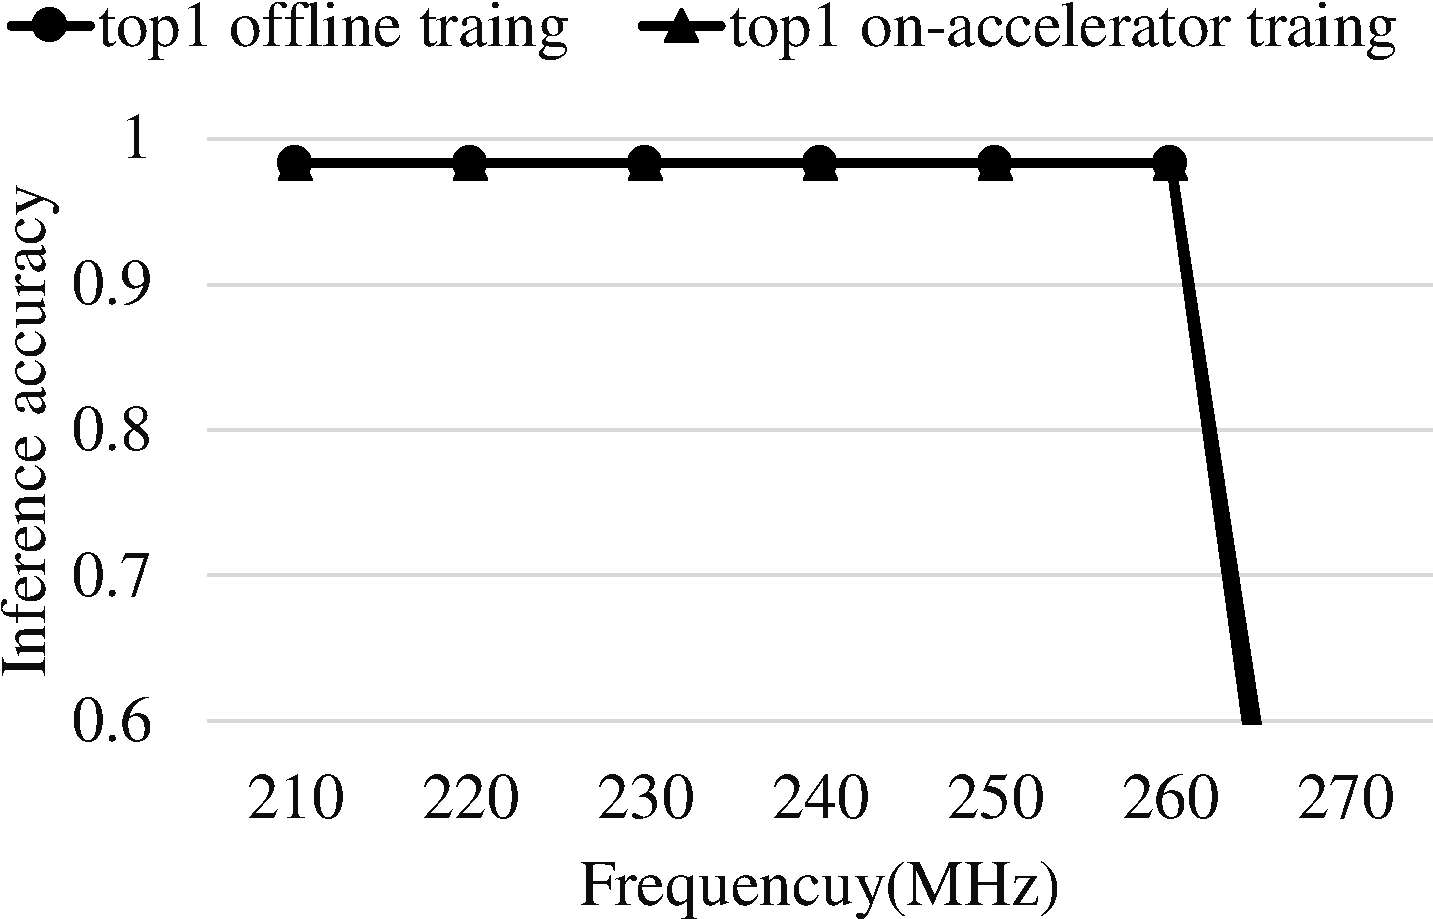
\includegraphics[width=0.65\linewidth]{accuracy_lenet}
	}
	\qquad
	\subfloat[AlexNet]{
                \label{fig:alexnet_accuracy}
                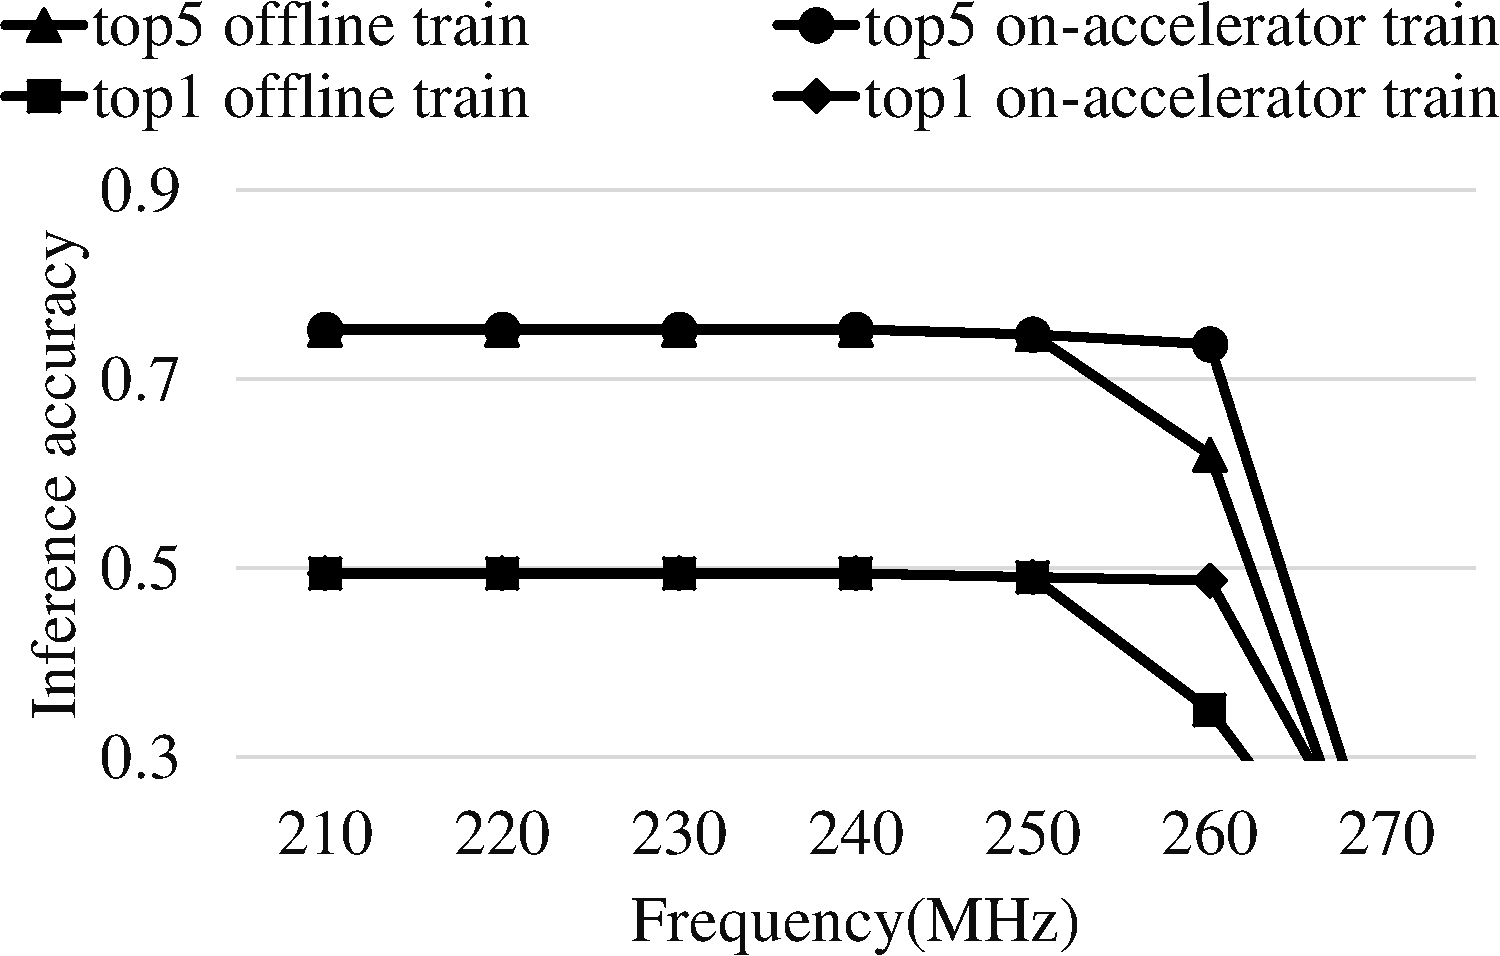
\includegraphics[width=0.65\linewidth]{accuracy_alexnet}
        }
	\qquad
	\subfloat[VGG-16]{
                \label{fig:vgg16_accuracy}
                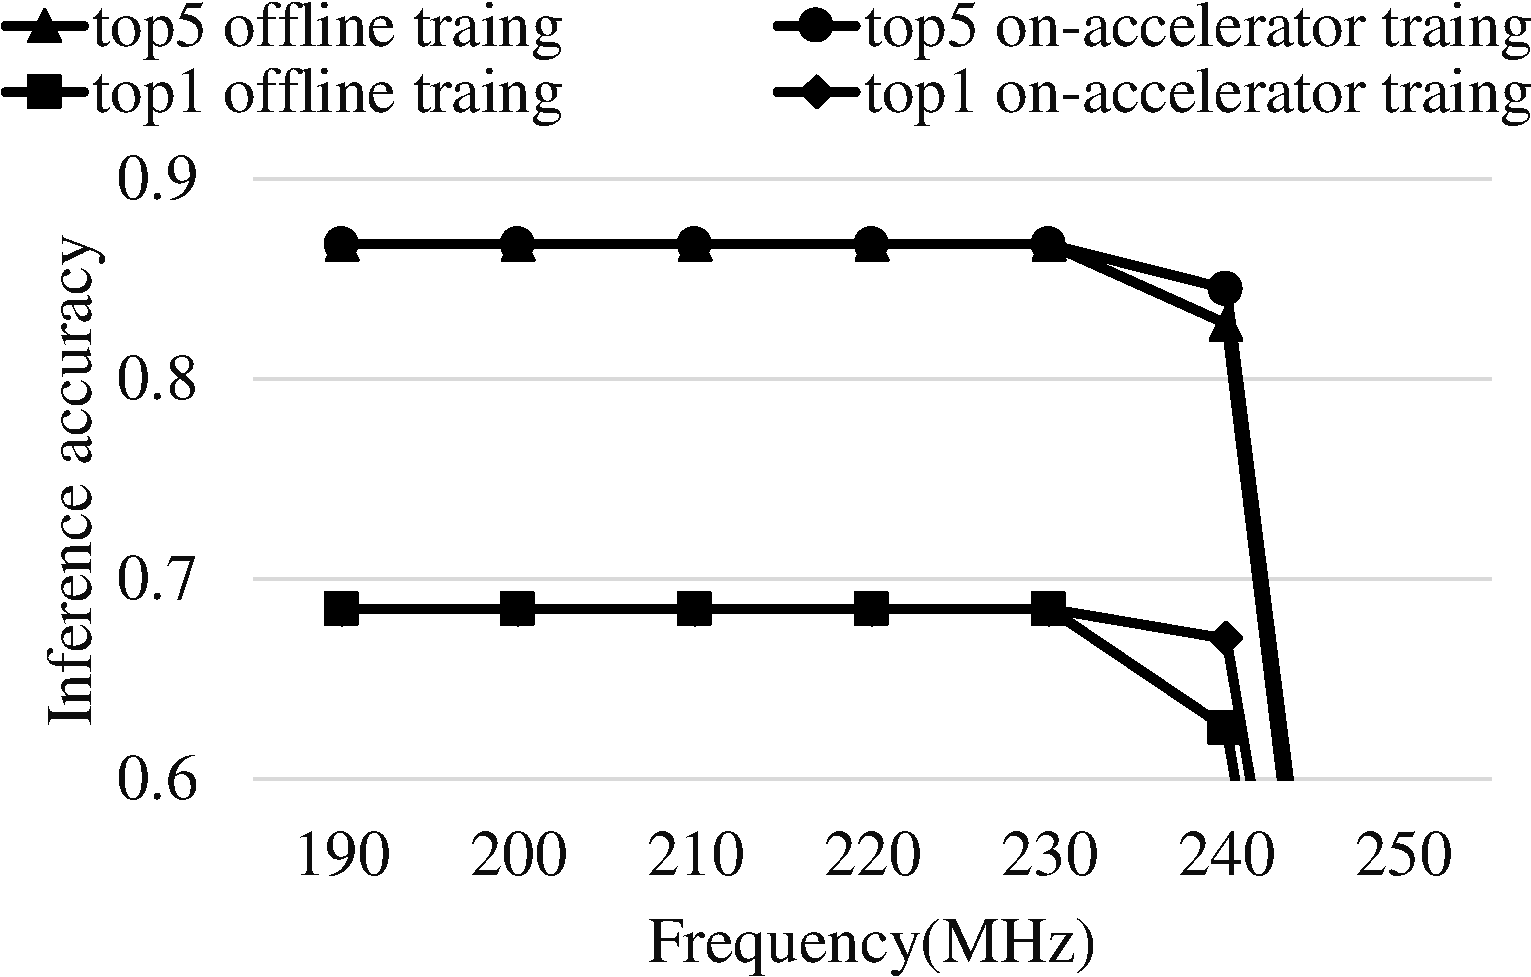
\includegraphics[width=0.65\linewidth]{accuracy_vgg16}
        }
        \qquad
	\subfloat[VGG-19]{
                \label{fig:vgg19_accuracy}
                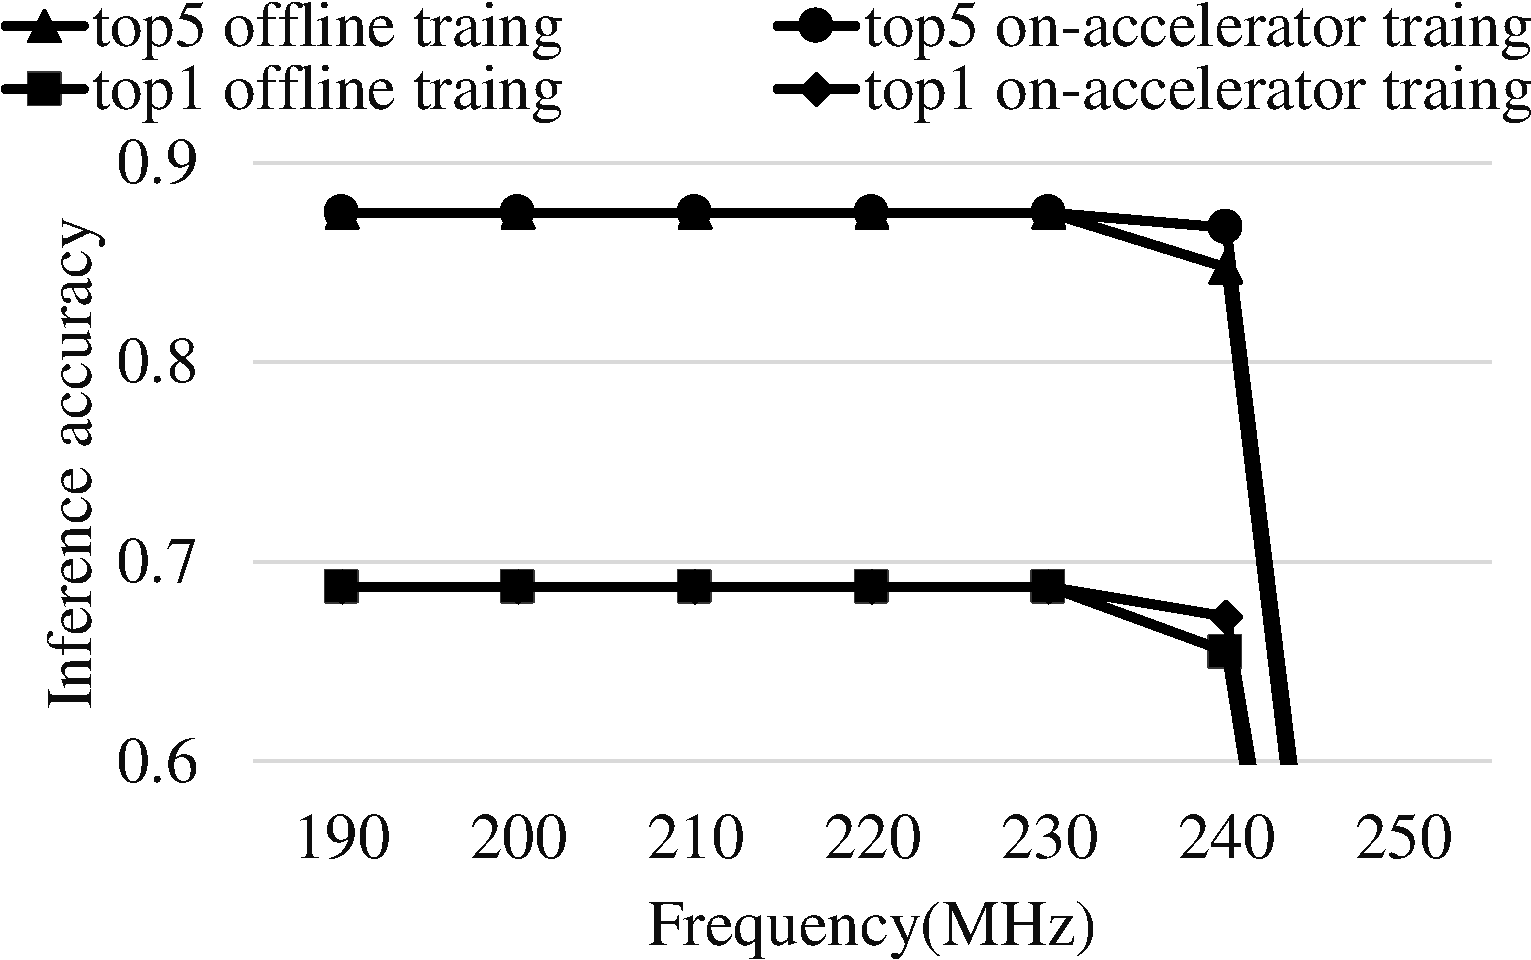
\includegraphics[width=0.65\linewidth]{accuracy_vgg19}
        }
	\caption{The prediction accuracy of the benchmark neural networks on accelerators with different overclocking}
        \label{fig:overclock-accuracy}
		\vspace{-1em}
\end{figure}

We further evaluate the normalized performance over the original CNN accelerators.
As given in Fig \ref{fig:relative_time_overclock}, the performance with the extreme accelerator 
overclocking achieves 1.25X speedup on average compared to the baseline design. 
We use EDP as the energy efficiency metric and compare the 
different overclocking configurations as exhibited in Fig \ref{fig:relative_energy_overclock}.
According to the figure, overclocking on FPGA based CNN 
accelerators achieves more significant energy efficiency improvement when 
compared to the performance improvement. A key reason is that 
the power consumption does not scale much with the clock frequency due to the 
relatively higher background power consumption. On the contrast, 
the performance which contributes more to the EDP metric scales 
much better. 

\begin{figure}
        \center{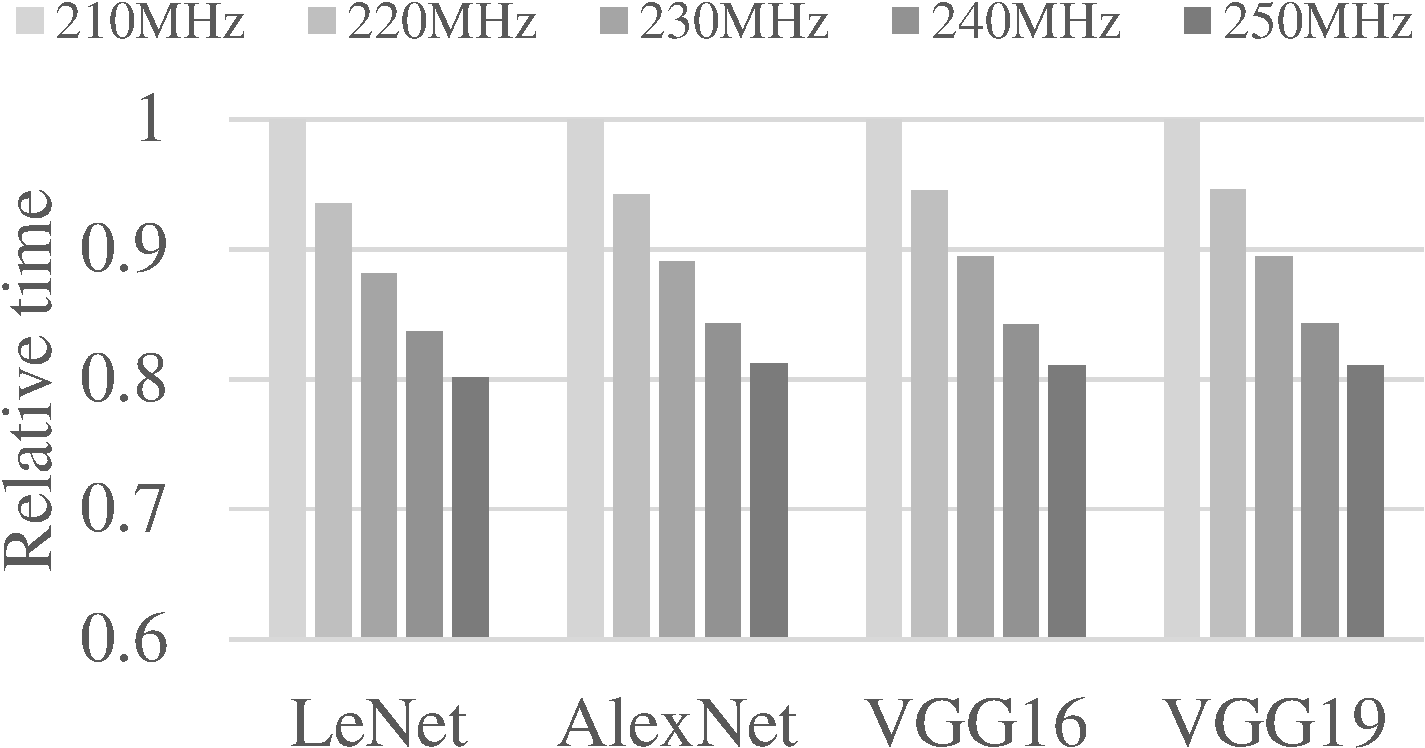
\includegraphics[width=0.65\linewidth]{relative_time_overclock}}
    \caption{Normalized performance of neural networks executed on CNN accelerators with different overclocking.}
\label{fig:relative_time_overclock}
\vspace{-1em}
\end{figure}

\begin{figure}
        \center{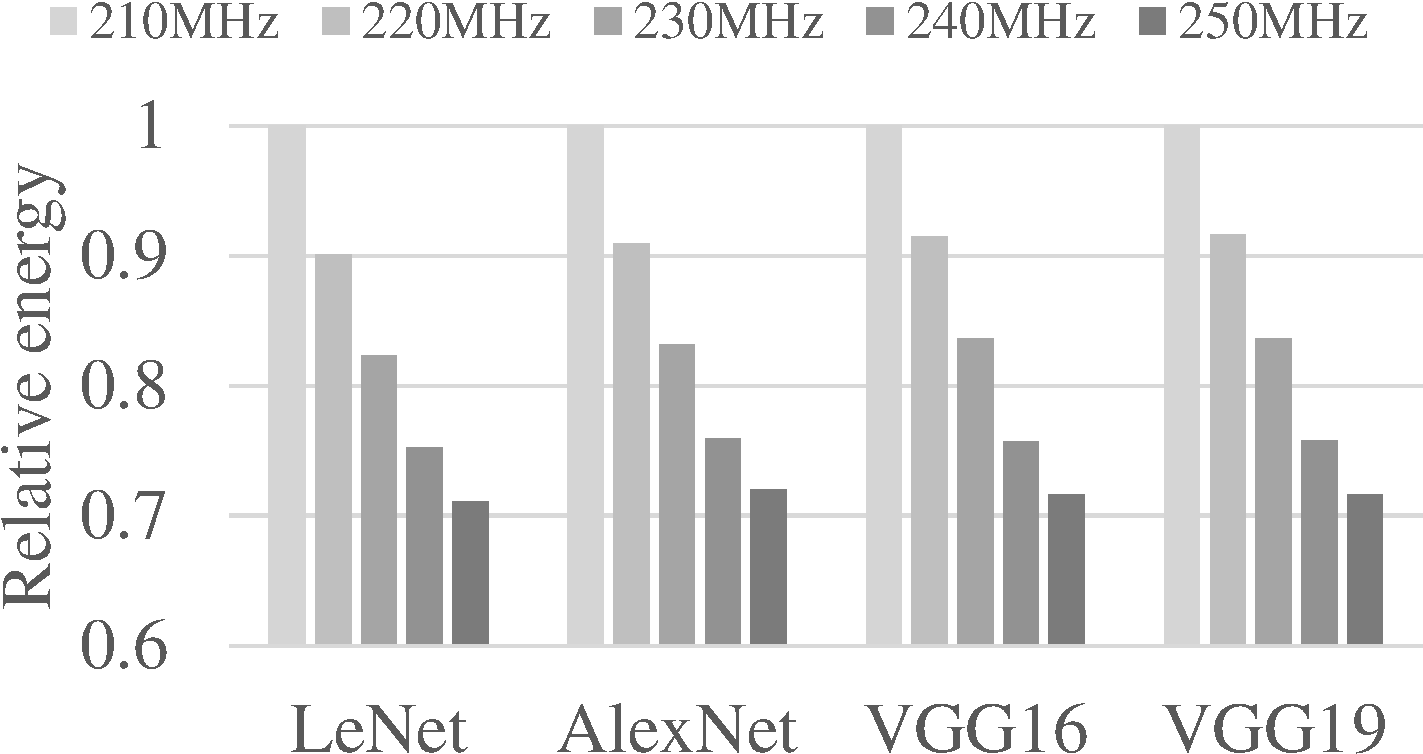
\includegraphics[width=0.65\linewidth]{relative_energy_overclock}}
    \caption{Normalized EDP of neural networks executed on CNN accelerators with different overclocking.}
\label{fig:relative_energy_overclock}
\vspace{-1em}
\end{figure}

In order to quantize the exact computing errors caused by overclocking, we 
particularly analyze the last layer output of the neural networks which 
is typically a vector. We compare it with the output without overclocking.
And we use the percentage of changed output data and the Euclidean distance 
of the output vectors to characterize the difference. 
The comparison is presented in Table \ref{tab:fr_ed}. It can be observed that 
computing errors can be completely hidden by the neural networks when the clock 
frequency is less than 240 MHz in the experiment. Moreover, the small Euclidean indicates that 
the computing error amplitude is relatively small though the percentage of 
the affected results is high when the clock is higher than 240 MHz.

\begin{table}
        \centering
        \vspace{-0.3em}
        \caption{Fault rate and Euclidean distance on the last output layer of the neural network}
        \label{tab:fr_ed}
        \vspace{-0.3em}
        \begin{tabular}{c|cccccc}
                \toprule
                Frequency(MHz) & 210 & 220 & 230 & 240 & 250 & 260 \\
                \midrule
                Euclidean distance & 0 & 0 & 0 & 0 & 35.2 & 104.8 \\
		\midrule
                Fault rate(\%) & 0 & 0 & 0 & 0 & 56.6 & 72.1 \\
                \bottomrule
        \end{tabular}
        \vspace{-1em}
\end{table}

\subsection{Optimization trade-offs}
As discussed in this paper, the timing error can be affected by many factors and it may change 
at runtime. There is no guarantee that the behavior of the CNN accelerator can keep stable even 
overclocking is just slightly higher than the original clock. We use the accelerator overclocked at the 
tipping point to perform the neural network computing. Then we keep measuring its 
prediction accuracy. As shown in Fig \ref{fig:stability}, we find that the accuracy is rather stable.
Although we still can not ensure the stability of the overclocked CNN accelerator, we can 
be sure that the probability of the severe errors such as accelerator hangup or considerable 
accuracy loss is rather low. As we did not observe the cases after processing 100000 pictures, 
we assume the probability of an severe error when processing an input picture is lower than 1/100000.

\begin{figure}
	\center{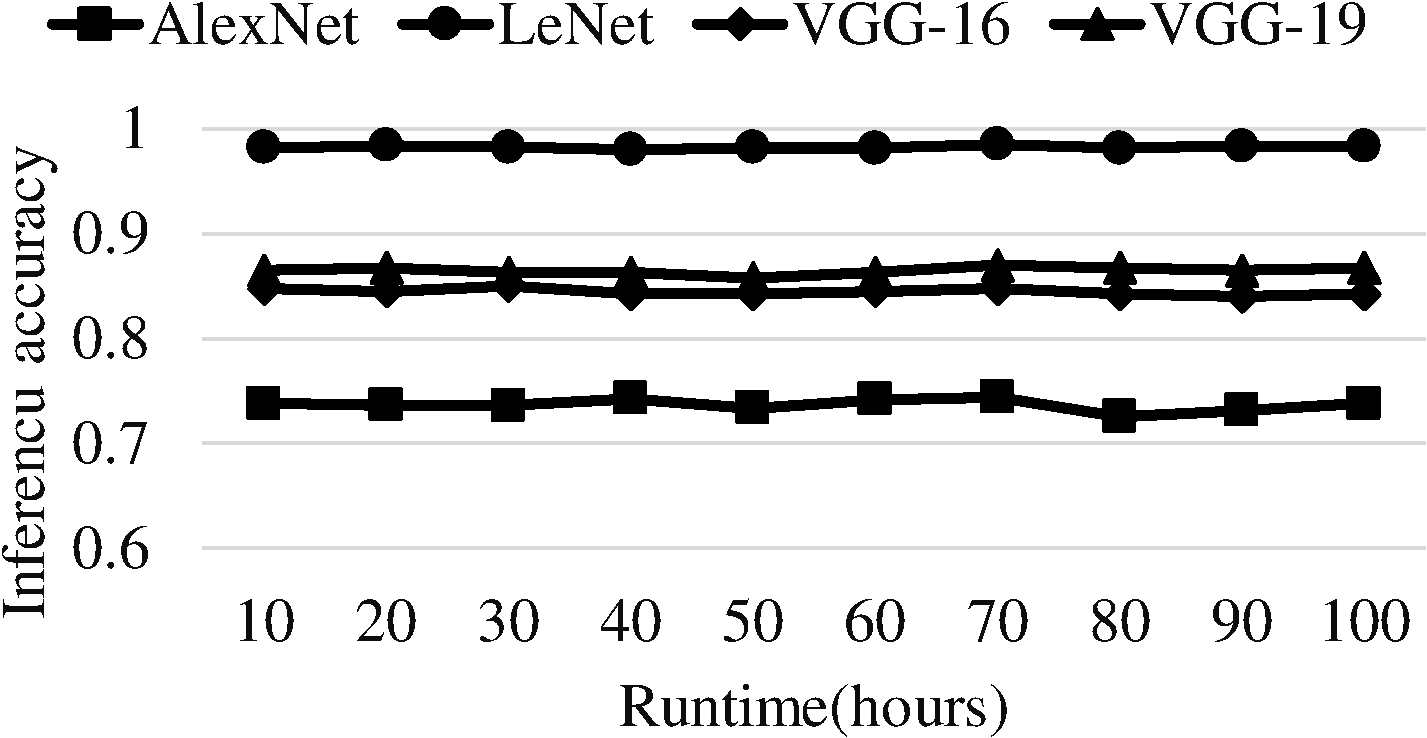
\includegraphics[width=0.65\linewidth]{stability}}
    \caption{Overclocking stability analysis}
\label{fig:stability}
\vspace{-1em}
\end{figure}

\begin{figure}
        \center{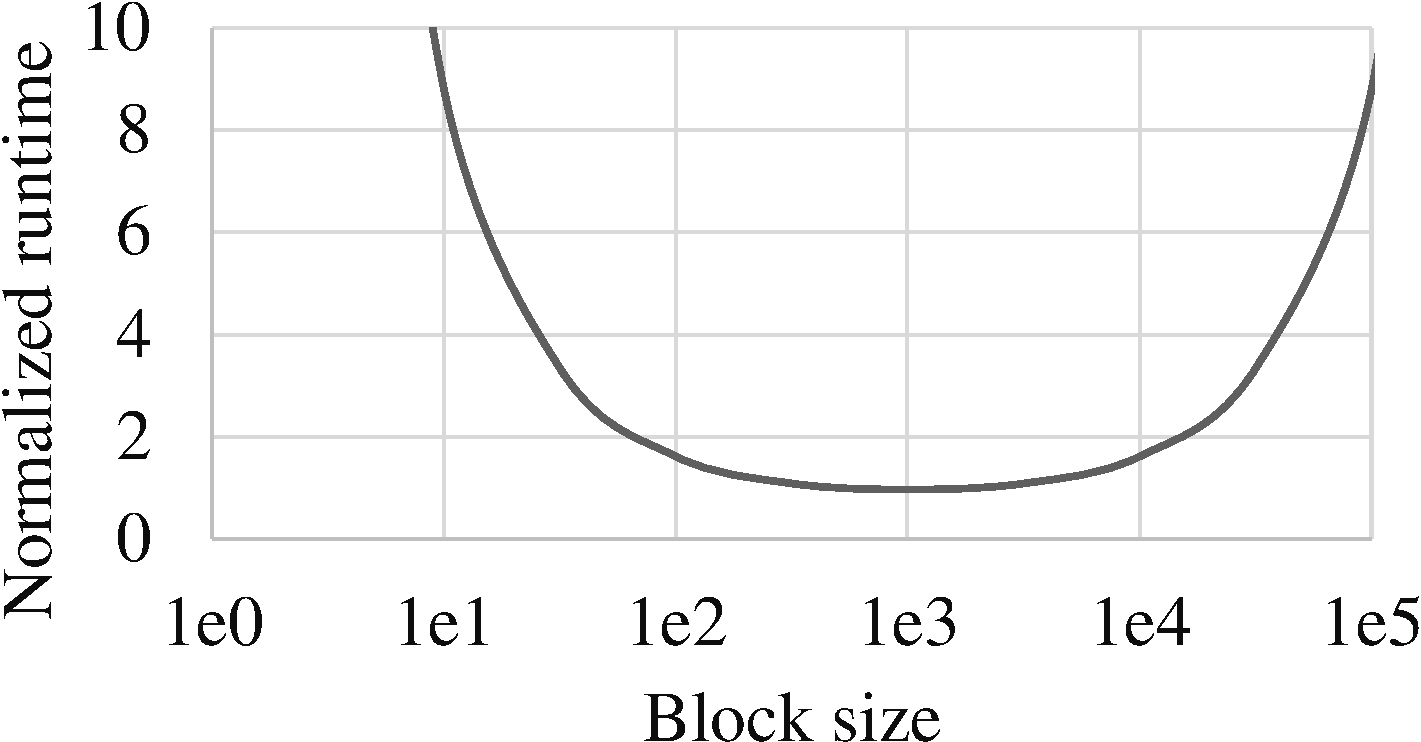
\includegraphics[width=0.65\linewidth]{cost_batch}}
    \caption{The relative overclocking runtime with different block size.}
\label{fig:cost_block}
\vspace{-1em}
\end{figure}

\begin{figure}
	\center{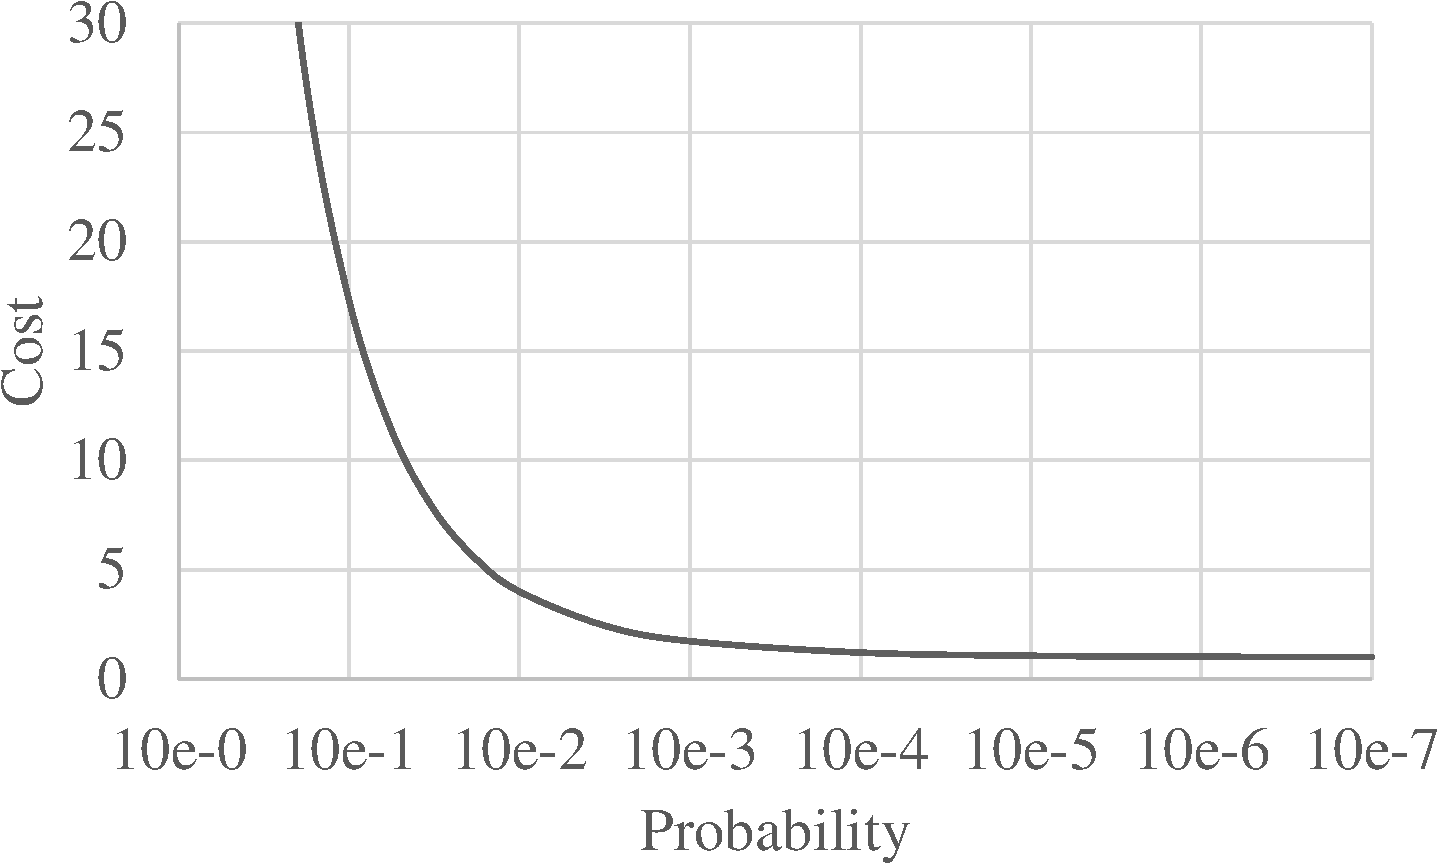
\includegraphics[width=0.65\linewidth]{cost_probability}}
    \caption{The relative overclocking runtime with different fault rate.}
\label{fig:cost_probability}
\vspace{-1em}
\end{figure}


With the severe errors, we need to invoke the checkpoint-based error recovery strategy. 
However, this strategy incurs cost including error detection and error recovery. 
We evaluate the overhead of the checkpoint-based strategy. 
A few parameters are critical to the overhead. One of them is the block size, which 
decides the granularity of checkpoint. One of them is the critical 
fault rate. It refers to the probability that CNN accelerator got severe errors 
when processing a single input figure. Another one is the reference data size.


Suppose reference data size is 100 and fault rate under 250 MHz is 1E-5. The relative runtime 
of overclocking over the normal design without overclocking is shown 
in Fig \ref{fig:cost_block}. When the block size is too big, the roll back cost will be 
too large and incurs additional runtime. When the block size is too small, the inserted 
reference data becomes non-trivial and the overall runtime also gets deteoriated. There is 
an optimal block size given specified fault rate and reference data size.
We also analyze the trend of the relative runtime under different fault rate.
As shown in Fig \ref{fig:cost_probability}, the relative runtime increases slightly at 
lower relative fault rate range but grows rapidly when the fault rate is larger than 1E-5.



\section{Related Work} \label{sec:relatedwork}
Despite of the performance and power advantages, the design 
productivity of developing FPGA applications remains low 
due to the lengthy compilation and complex application-specific 
customization. And it has become the major obstacle 
that hinders the wide adoption of FPGAs as commodity computing devices. 
The community from both the industry and academia have developed 
many different methods from diverse angles to tackle the problem. 
These methods can be roughly classified into three categories. 
The first category mainly focuses on improving the low-level 
implementation tools. A number of approaches such as making 
quality/runtime trade-offs \cite{mulpuri2001runtime}, parallel 
compilation \cite{moctar2014parallel, goeders2011deterministic, altera-pc, 
xilinx-pc} and using hard-macro techniques \cite{lavin2013improving, 
korf2011automatic} have been explored from this angle. The second 
category mainly centers the HLS design flow while the third one 
primarily relies on the overlay concept. They later two categories 
will be detailed in the following sections.

\subsection{High-Level Synthesis} 
With many years of continuous endeavor, a number of tools have emerged as 
mature solutions for HLS \cite{VivadoHLS, Legup, zhang2008autopilot}. They typically 
allow designers to express hardware designs using high-level  
description languages such as C, C++ etc. and also enable evaluation of different 
design choices using pragmas or directives. Indeed, they significantly improve 
the design productivity compared to the conventional hardware design flow using 
hardware description languages. However, when considering the overall design 
productivity of developing hybrid software-gateware applications, HLS is 
only addressing part of the problem, as the lengthy low-level compilation 
including synthesis, mapping, placing and routing remains a bottleneck for 
an application designer \cite{ROB2014, capalija2014tile}.

Customizing the generated hardware specifically to an user 
application is also time-consuming for designers and thus critical to the design 
productivity. A number of algorithms such as generic algorithms 
relied on local-search techniques \cite{schafer2009adaptive, 
sengupta1997genetic}, learning-based methods \cite{onlinecustomization, 
carrion2012machine}, divide and conquer algorithm \cite{DCcustomization} 
and a calibration free algorithm \cite{RCcustomization} etc. have been developed 
to perform the DSE on top of HLS tools. The algorithms can efficiently help automate the 
customization or DSE process. However, the algorithms must rely on HLS tools 
to estimate the implementation information such as implementation frequency, 
overhead or power for the corresponding customization. While the hardware generated 
can be irregular and may vary dramatically, thus the accuracy of the estimation 
especially on implementation frequency and power can be rather limited, which may
fail to optimize an HW/SW co-design problem.  

\subsection{Overlay Architectures}
Overlay architecture which is a virtual intermediate architecture overlaid on 
top of off-the-shelf FPGA is increasingly applied as a way to address the 
productivity challenge. 

Various overlays with diverse configuration granularities and flexibility 
ranging from virtual FPGAs \cite{Grant2011Malibu, ZUMA2012}, 
array-of-FUs \cite{mesh-FUs,ferreira2011fpga}, soft 
CGRA \cite{kissler2006dynamically, scgra-orig}, soft GPU \cite{Guppy2012GPU-Like}, 
vector processors\cite{Yiannacouras2009FPS, MXP2013} to 
configurable processors or multi-core processors \cite{unnikrishnan2009application, 
MARC2010, Yiannacouras2007Exploration, Capalija2009coarse-grain, OCTAVO2012, iDEA2012} 
have been developed over the years. SCGRA overlay provides unique 
advantages on compromising hardware implementation 
and performance for compute intensive nested loops as demonstrated 
by numerous ASIC CGRAs \cite{tessier2001reconfigurable, compton2002reconfigurable}.
Most importantly, it allows both rapid compilation by taking advantage of 
the overlays' tiling structure \cite{ROB2014} and efficient bitstream 
reuse within the design iterations of an application \cite{scgra-orig}, 
thus it is particularly promising for high productivity nested loop acceleration.

Despite of the promising potential, a complete automatic customization 
framework that enables application-specific optimization is still highly 
anticipated for the sake of design productivity and performance. 
The authors in \cite{colinheart} developed an SCGRA topology customization method 
using genetic algorithm and showed the potential benefits of the SCGRA 
overlay customization. However, the rest system design parameters such as 
on chip buffer size, loop unrolling factor etc. are not covered. 

Indeed, SCGRA overlays have many similarities in terms of array structure 
and scheduling algorithm with ASIC CGRAs. Nevertheless, ASIC CGRAs emphasize 
more on configuration capability and limited customization is allowed due 
to the overhead constraints \cite{zhou2014application, miniskar2014retargetable} 
while SCGRA overlays allow more intensive architectural customization 
because of the FPGA's inherent programmability. Moreover, hardware resources such as 
DSP blocks and RAM blocks available on FPGAs are discrete, which results in different 
design constraints for SCGRA overlay customization as well. 

By utilizing the SCGRA overlay as the backbone of the FPGA accelerator, 
a complete nested loop acceleration framework 
targeting CPU-FPGA system is developed. It supports intensive application-specific
customization including the overlay architectural customization, 
the compilation customization and communication interface customization 
for various design goals. When the customized design parameters are determined, 
corresponding hardware accelerator and software can be compiled to the target 
CPU-FPGA system rapidly eventually providing a push-button solution for a nested loop 
acceleration. 


 
\section{Conclusion} \label{sec:Conclusion}
In this work, we propose to replace the forward computing on GPPs with accelerator 
computing during training and have both the computing 
errors and the application data learned in the neural network models. 
In addition, we opt to protect critical neural layers to reduce the negative 
influence of computing errors.  
With the proposed resilient neural network training, 
the prediction accuracy of the retrained neural network models improves significantly 
when computing errors appear. 


%\appendix
%\section{Acknowledgement}

%\begin{acks}
%  The authors would like to thank Sam Ho for providing the suggestions on
%  HLS design debugging and optimization as well as the SDAccel usage. 

%\end{acks}


\bibliographystyle{IEEEtran}
\bibliography{refs} 


% trigger a \newpage just before the given reference
% number - used to balance the columns on the last page
% adjust value as needed - may need to be readjusted if
% the document is modified later
%\IEEEtriggeratref{8}
% The "triggered" command can be changed if desired:
%\IEEEtriggercmd{\enlargethispage{-5in}}

% references section

% can use a bibliography generated by BibTeX as a .bbl file
% BibTeX documentation can be easily obtained at:
% http://mirror.ctan.org/biblio/bibtex/contrib/doc/
% The IEEEtran BibTeX style support page is at:
% http://www.michaelshell.org/tex/ieeetran/bibtex/
%\bibliographystyle{IEEEtran}
% argument is your BibTeX string definitions and bibliography database(s)
%\bibliography{IEEEabrv,../bib/paper}
%
% <OR> manually copy in the resultant .bbl file
% set second argument of \begin to the number of references
% (used to reserve space for the reference number labels box)
%\begin{thebibliography}{1}

%\bibitem{IEEEhowto:kopka}
%H.~Kopka and P.~W. Daly, \emph{A Guide to \LaTeX}, 3rd~ed.\hskip 1em plus
%  0.5em minus 0.4em\relax Harlow, England: Addison-Wesley, 1999.

%\end{thebibliography}




% that's all folks
\end{document}


